% Generated by thesis/ch7/exp2/make_assets.py -- do not edit by hand.
\begin{figure}[tbp]
  \centering
  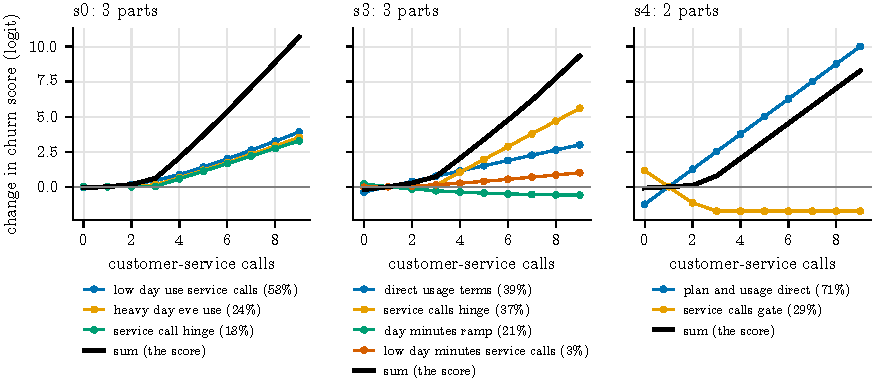
\includegraphics[width=\textwidth]{figures/exp2/exp2-churn-calls-parts}
  \caption{Churn: one signal, three realisations. The score's response to customer-service calls (relative to 1 call), split into the explanation parts that carry it; black: their sum, the score's response. Legend: each part's share of the response's variance.}
  \label{fig:exp2-churn-calls-parts}
\end{figure}
